\iffalse
The new generation of the collaborative robots allow the use of small robot arms working in an asynchronous or synchronous fashion with human workers.  Such an example of the collaborative robot is the YuMi robot, dual 7-DOF robot arms designed for precise manipulation of small parts better known in computer vision as rigid body. For further acceptance of such robots in the industry, some methods and sensors systems have to be developed to allow them to pick parts without the position of the part being known in advance, just as humans do.
This thesis is focused on the implementation of an algorithm for determing the positition of the known parts. We first deal with a robot-camera calibration, then  we propose a method to obtain the ground truth position of known parts. As step in between a 3D model of the known part needs to be created.
\fi


	\bibitem{planarTargets}
		B. Atcheson, F. Heide, and W. Heidrich,
		"CALTag: High Precision Fiducial Markers for CameraCalibration" in: Vision, Modeling, and Visualization, 2010, \url{https://pdfs.semanticscholar.org/2dba/e046717b058382a5a04f800405f92d040200.pdf}.






\begin{figure}[!h]
\begin{center}
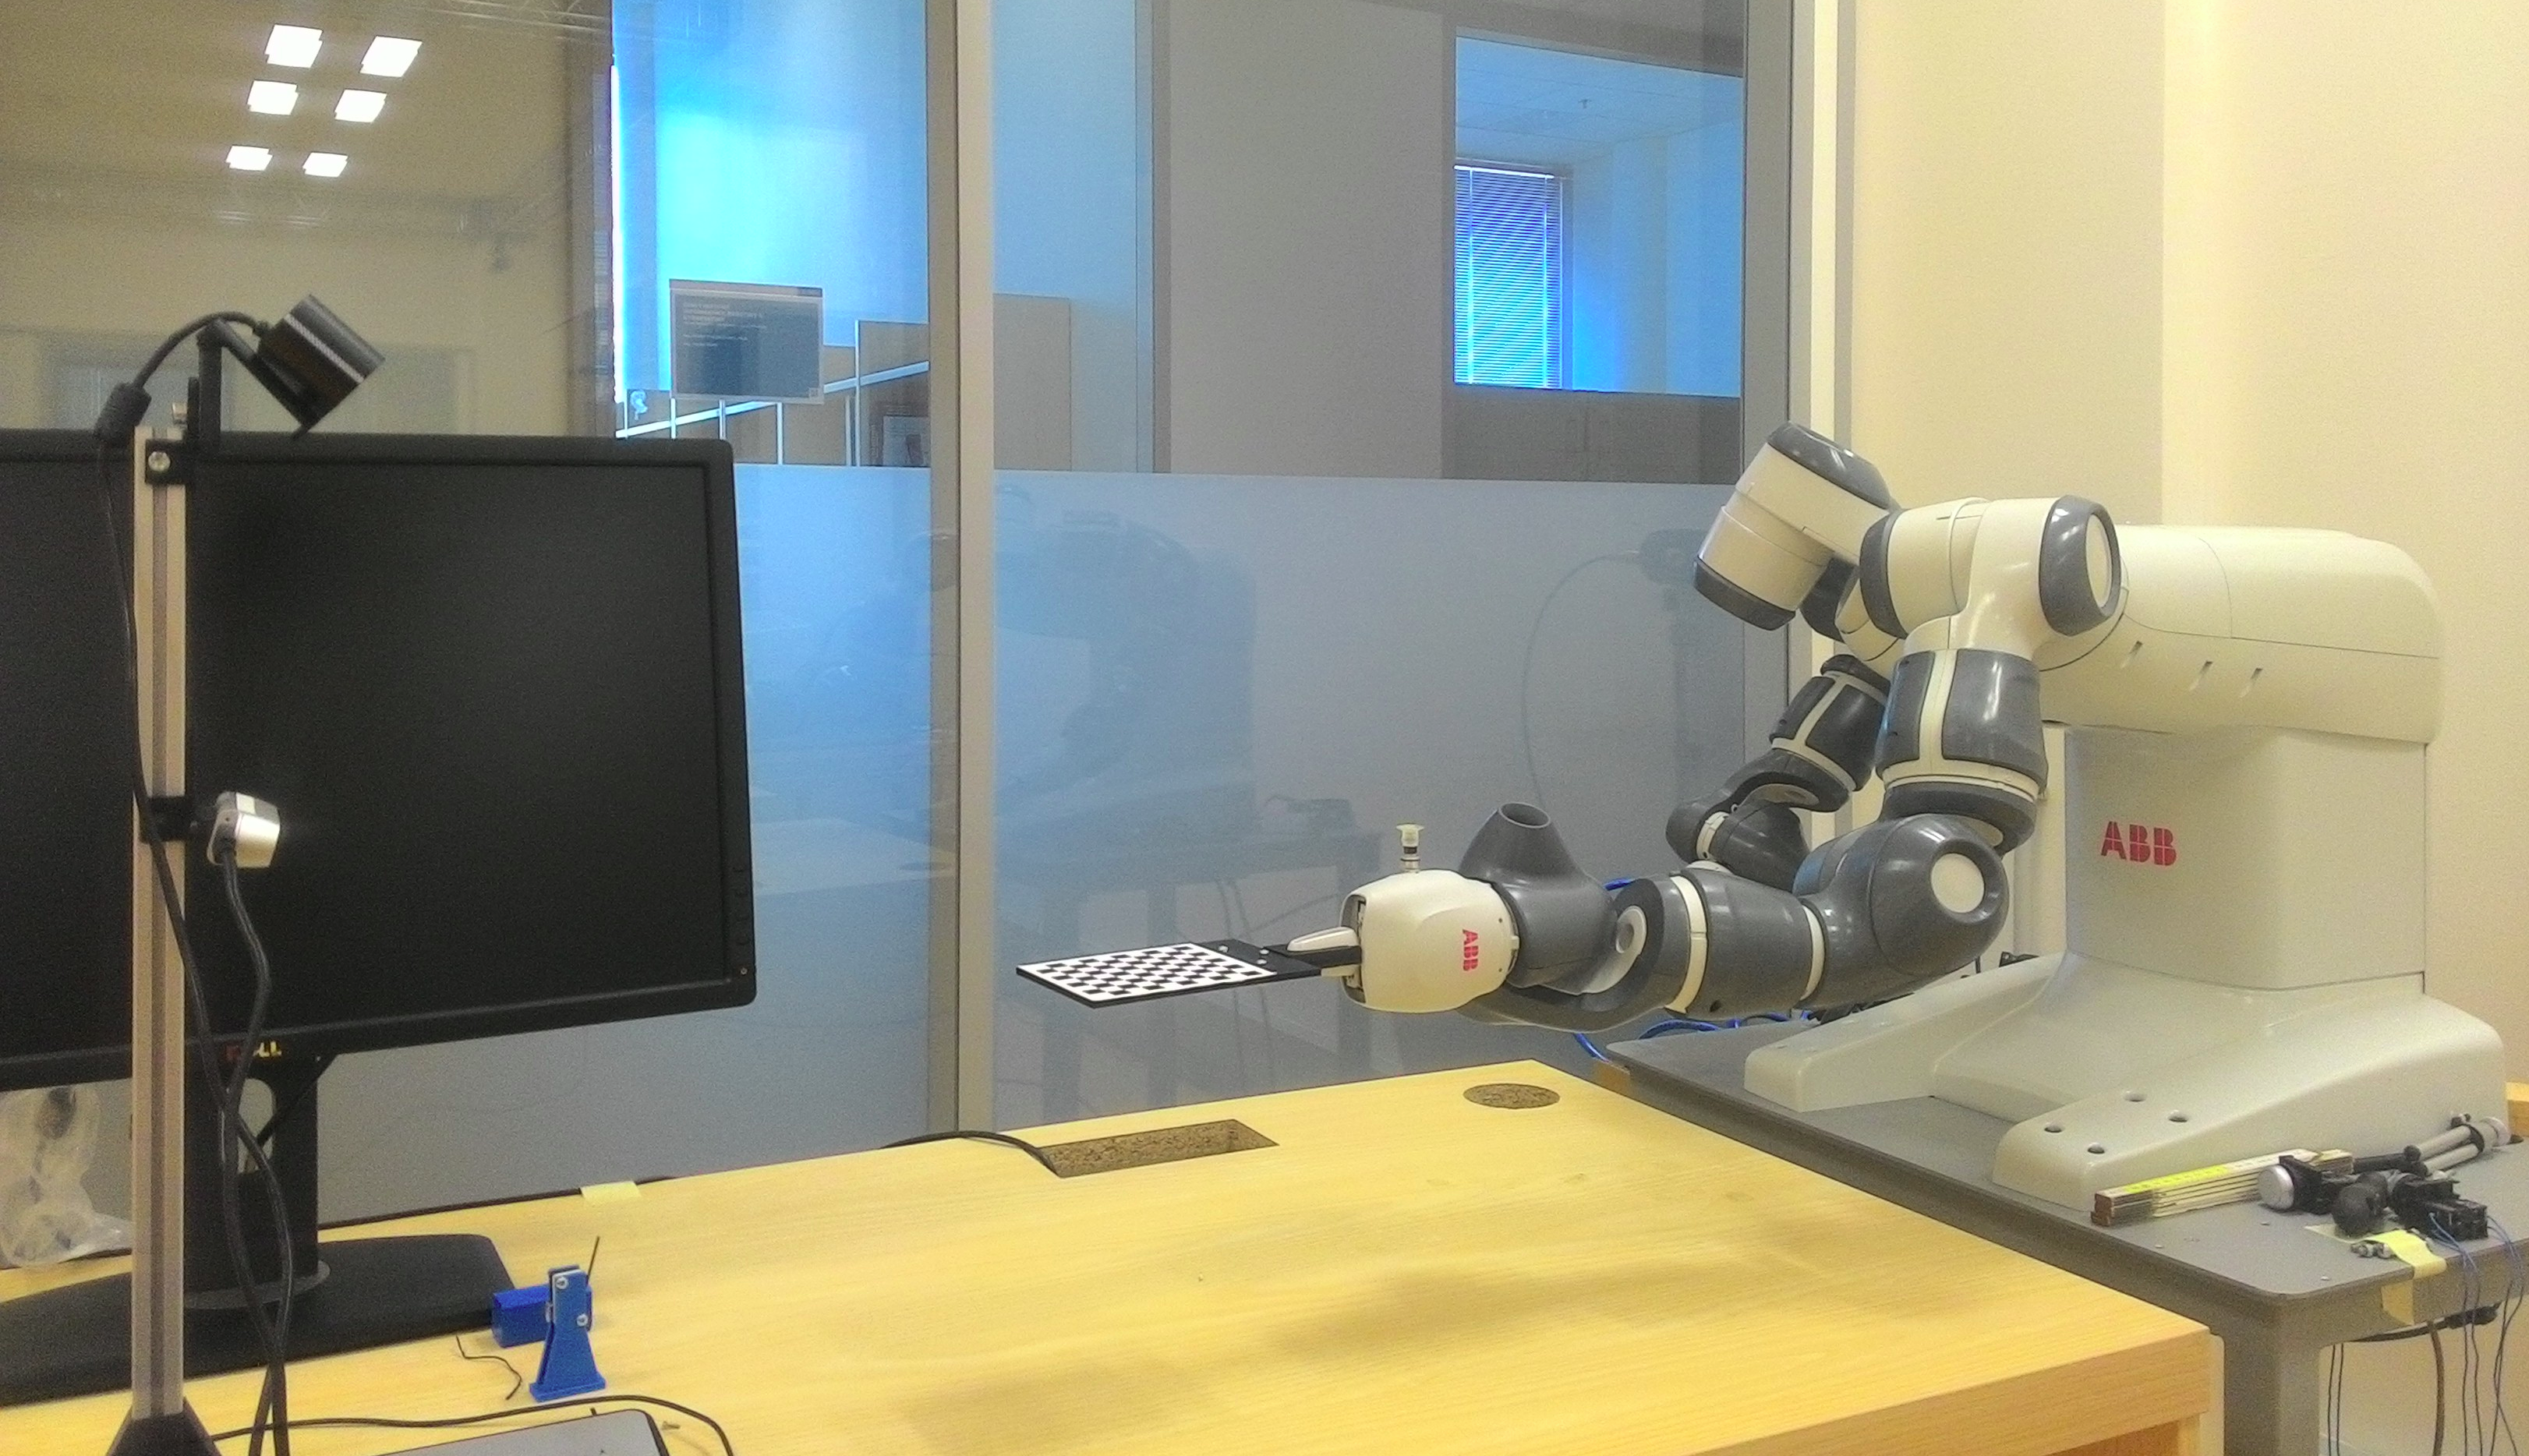
\includegraphics[width=4in]{figures03/setup.png}
\caption{Overview of the setup, a ABB YUMI robot with a gripper holding the calibration plate. The camera is fixed around the robot workspace and pointed at the checkerboard}%\cite{temp2}}
\label{fig:setup}
\end{center}
\end{figure}



In \ref{caltar} methods to estimate the position of the camera relative to a calibration targets have been briefly reviewed. This position data, plus the pose of calibration plate relative to the robot base frame are used to calculate the pose of the camera coordinate system relative to the robot base coordinate system with the help of TF ROS packages.




In Figure \ref{fig:setup} an example setup is given of a robot arm with a gripper holding a calibration plate with a the 6x9  checkerboard sticks on it. The robot arm can move the calibration plate around the robot workspace where a camera is fixed and takes a sequence of pictures from different movement.



